% Shared rehabilitation results for the paper and technical report.
\subsection{Rehabilitation and Limits of the 2PT Excess Entropy}
\label{sec:2pt_rehabilitation}

We reanalyzed the existing final-$100\tau$ velocity records of all 24 replicas using a corrected classical two-phase thermodynamic (2PT) estimator. The revised spectral construction follows Sun \emph{et al.}~\cite{Sun2017}, with the equal-partial-volume mixture approximation discussed by Lai \emph{et al.}~\cite{Lai2012}. Each species is assigned $\bar V_i=1/\rho$; equal nominal diameters do not establish equality of actual partial volumes in these charged, dispersion-diverse liquids. The primary gas/solid partition exponent is $\delta=1$; the published LJ value $\delta=1.5$ is an unfitted sensitivity. Neither partition, reference volume, nor entropy offset is adjusted to match thermodynamic integration (TI).

The calculation corrects the density scaling and prefactor of the normalized diffusivity ($\Delta\propto D\sqrt{m/T}\rho^{1/3}$), weights gas entropy by its gas-like fraction, and subtracts the classical ideal-mixture reference consistently. The complete finite-record autocorrelation, in the common system-COM frame, is Gaussian-tapered with primary width $10\tau$. Its spectrum spans the full Nyquist band and is normalized by measured $C(0)$ to three modes per particle; raw target-temperature mode counts are retained as a diagnostic. The gas Lorentzian and its entropy tail are integrated analytically to infinity. The residual spectrum is kept signed as revised-2PT bookkeeping, rather than clipped to a positive ``solid population.'' This partition is not a literal count of free ions or bound oscillators.

Seven analytic checks pass, including the standard fluidicity polynomial, unit invariance, a solvable VACF/Green--Kubo limit, the Lorentzian entropy tail, the dilute-gas limit, and classical-reference and label/mixing cancellation. Normalization, reconstruction, and independence of the arbitrary classical phase-space constant hold to floating-point precision. Mechanically identical labels are pooled before the nonlinear entropy estimate. For all three actual U4/L5 pairs, matched retained particle IDs have identical COM-corrected velocity hashes, VACFs, and resulting 2PT entropies. Separately processing the label samples gives a difference $+0.00062k_B$, interval $[-0.00428,0.00553]k_B$, consistent with sampling. State-mean pooled-probe spectral diffusivities agree with the full-production MSD coefficients within $2.6\%$.

\begin{figure*}[t]
\centering
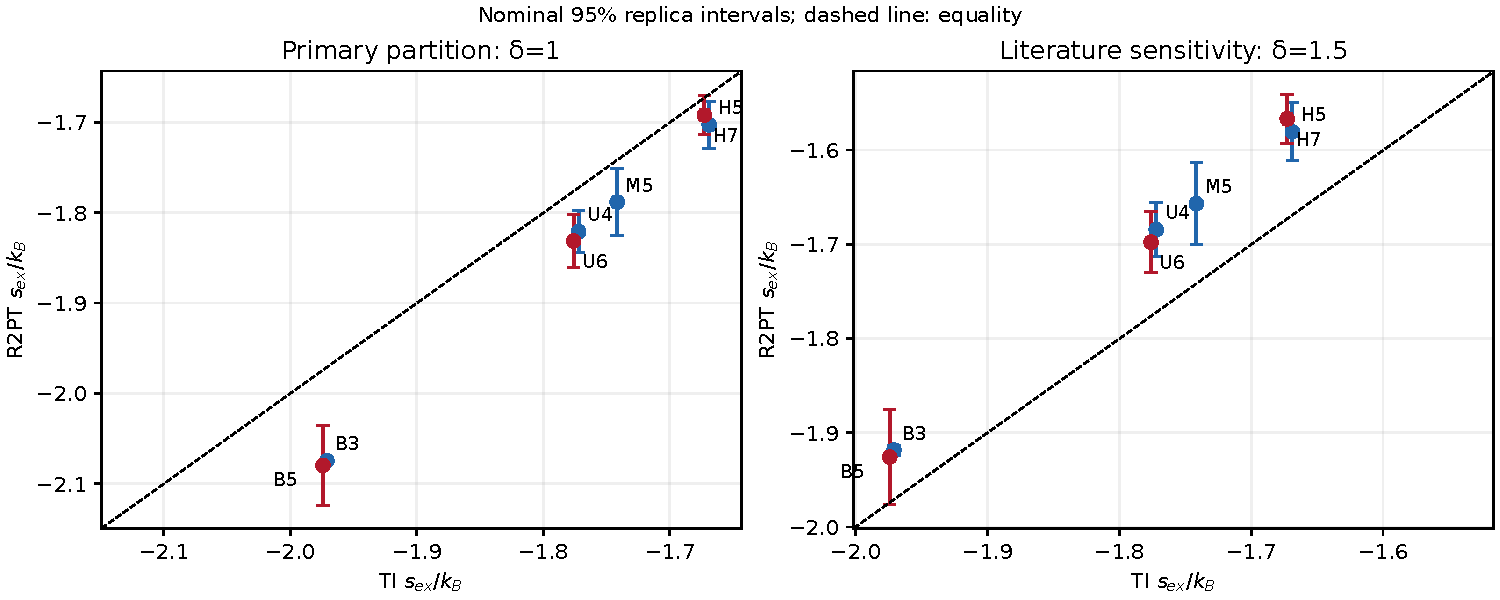
\includegraphics[width=\textwidth]{figures/component_2pt_validation.pdf}
\caption{Corrected classical revised-2PT excess entropy against TI for the seven mechanically distinct mixtures. L5 duplicates U4 in transport and is omitted. Bars are nominal 95\% absolute-state replica intervals; dashed lines denote equality. The left panel uses the primary partition $\delta=1$, and the right panel the unfitted literature sensitivity $\delta=1.5$. Internal consistency does not remove composition-dependent thermodynamic bias.}
\label{fig:2pt_validation}
\end{figure*}

These successes rehabilitate the implementation, but not its quantitative thermodynamic accuracy across compositions (Fig.~\ref{fig:2pt_validation}). For B3 the primary estimate is $-2.07445k_B$, compared with TI $-1.97101k_B$: the approximately $3.4k_B$ discrepancy of the archived $-5.376k_B$ result is reduced to $0.10344k_B$. Primary absolute biases range from about $-0.019$ to $-0.105k_B$, with all nominal paired bias intervals below zero. B3, B5, and U6 exceed the prespecified practical mean-bias tolerance $0.05k_B$. Thus the remaining error is composition dependent and comparable to the controlled entropy signal; a constant offset is insufficient.

% Generated by generate_component_study_assets.py; do not edit numbers by hand.
\begin{table*}[t]
\centering
\caption{Controlled excess-entropy increments from TI and corrected classical revised 2PT. All entropy quantities are per particle in $k_B$. Bias is the paired difference between the 2PT and TI increments; brackets are nominal 95\% Student-$t$ intervals from three independent replica pairs (two degrees of freedom), without multiplicity correction. The primary partition is $\delta=1$; $\delta=1.5$ is an unfitted sensitivity.}
\label{tab:2pt_contrasts}
\small
\resizebox{\ifdim\width>\textwidth\textwidth\else\width\fi}{!}{%
\begin{tabular}{llrrr}
\toprule
Comparison & Partition & TI $\Delta s_{\rm ex}/k_B$ & 2PT $\Delta s_{\rm ex}/k_B$ & Bias [95\% CI] \\
\midrule
H5/U4 & $\delta=1$ & 0.10322 & 0.11818 & $+0.01496\;[-0.00544,+0.03536]$ \\
H5/U4 & $\delta=1.5$ & 0.10322 & 0.10397 & $+0.00075\;[-0.02175,+0.02326]$ \\
H7/U6 & $\delta=1$ & 0.10331 & 0.13927 & $+0.03596\;[+0.01501,+0.05692]$ \\
H7/U6 & $\delta=1.5$ & 0.10331 & 0.13086 & $+0.02755\;[+0.00705,+0.04805]$ \\
\bottomrule
\end{tabular}}
\end{table*}


For H5/U4, primary 2PT gives $\Delta s_{\rm ex}=0.11818k_B$ versus TI $0.10322k_B$, a point bias $+0.01496k_B$ (Table~\ref{tab:2pt_contrasts}). This meets the practical point-bias tolerance $0.02k_B$ and is statistically consistent with zero bias, but the wide interval does not establish equivalence within that tolerance. For H7/U6, the estimate is $0.13927k_B$ versus $0.10331k_B$, an approximately $35\%$ overestimate; its bias interval $[0.01501,0.05692]k_B$ excludes zero. The $\delta=1.5$ partition improves the first increment to $0.10397k_B$ but still overestimates the second at $0.13086k_B$. Agreement for one pair does not validate a partition for all compositions.

The discrepancies survive sensitivity checks. State-mean entropy spans over taper widths 5, 10, and $20\tau$ are $0.011$--$0.022k_B$; first/last-half record shifts reach $0.012k_B$. Frequency-grid refinement changes means by less than $0.00002k_B$, and sampling-interval decimation changes them by at most $0.0022k_B$. Illustrative volume-conserving $\pm10\%$ partial-volume perturbations shift means by at most $0.0032k_B$, without establishing that the equal-volume approximation is exact. Positive-part clipping would add modes: the signed negative residual represents approximately 2.3--3.9\% of the total mode weight in primary species spectra. The corrected bookkeeping avoids this artifact, but cannot eliminate the model dependence of the gas/solid partition.

We therefore retain TI as the entropy coordinate in the Rosenfeld analysis. Corrected 2PT and the underlying VACFs remain useful dynamical diagnostics, but species spectral allocations are not independently measured partial molar entropies. Because diffusion enters the zero-frequency spectrum and fluidicity construction, a 2PT--diffusion correlation is not an independent confirmation of entropy-driven enhancement. Probe fluidicity rises from about 0.530 in B3 to 0.569 in H5, consistent with increased low-frequency motion. However, the mean probe VACFs remain positive over the first $\tau$; a pronounced early negative backscattering minimum is not supported. Association populations and residence times, rather than a literal interpretation of the 2PT partition, are needed to test local-caging mechanisms.
